%------------------------------------------------------------------------
% Chapter:  Frames
%------------------------------------------------------------------------

\chapter{Using frames \label {frame}}

In this chapter we will introduce the usage of frames that enable
{\it KUPLOT} to display more than one view graph in a single plot. A
detailed description of all frame related commands is available as
part of the online help which can be accessed by entering {\tt help
frames} at the input prompt.

%------------------------------------------------------------------------

\section{Introduction \label{frame-int}}

Frames enable {\it KUPLOT} to display multiple view graphs within a
single plot. The layout is defined by the user. A simple example with
two graphs being plotted on a single page is shown in Figure
\ref{fra-fig1}. Let us have a look at the macro file that was used to
create the figure and learn step by step how to use this
feature of {\it KUPLOT}. Note that the line numbers shown in the
listing below are used for easy reference in this manual and are not
part of the actual macro file.

\begin{figure}[!b]
   \centering
   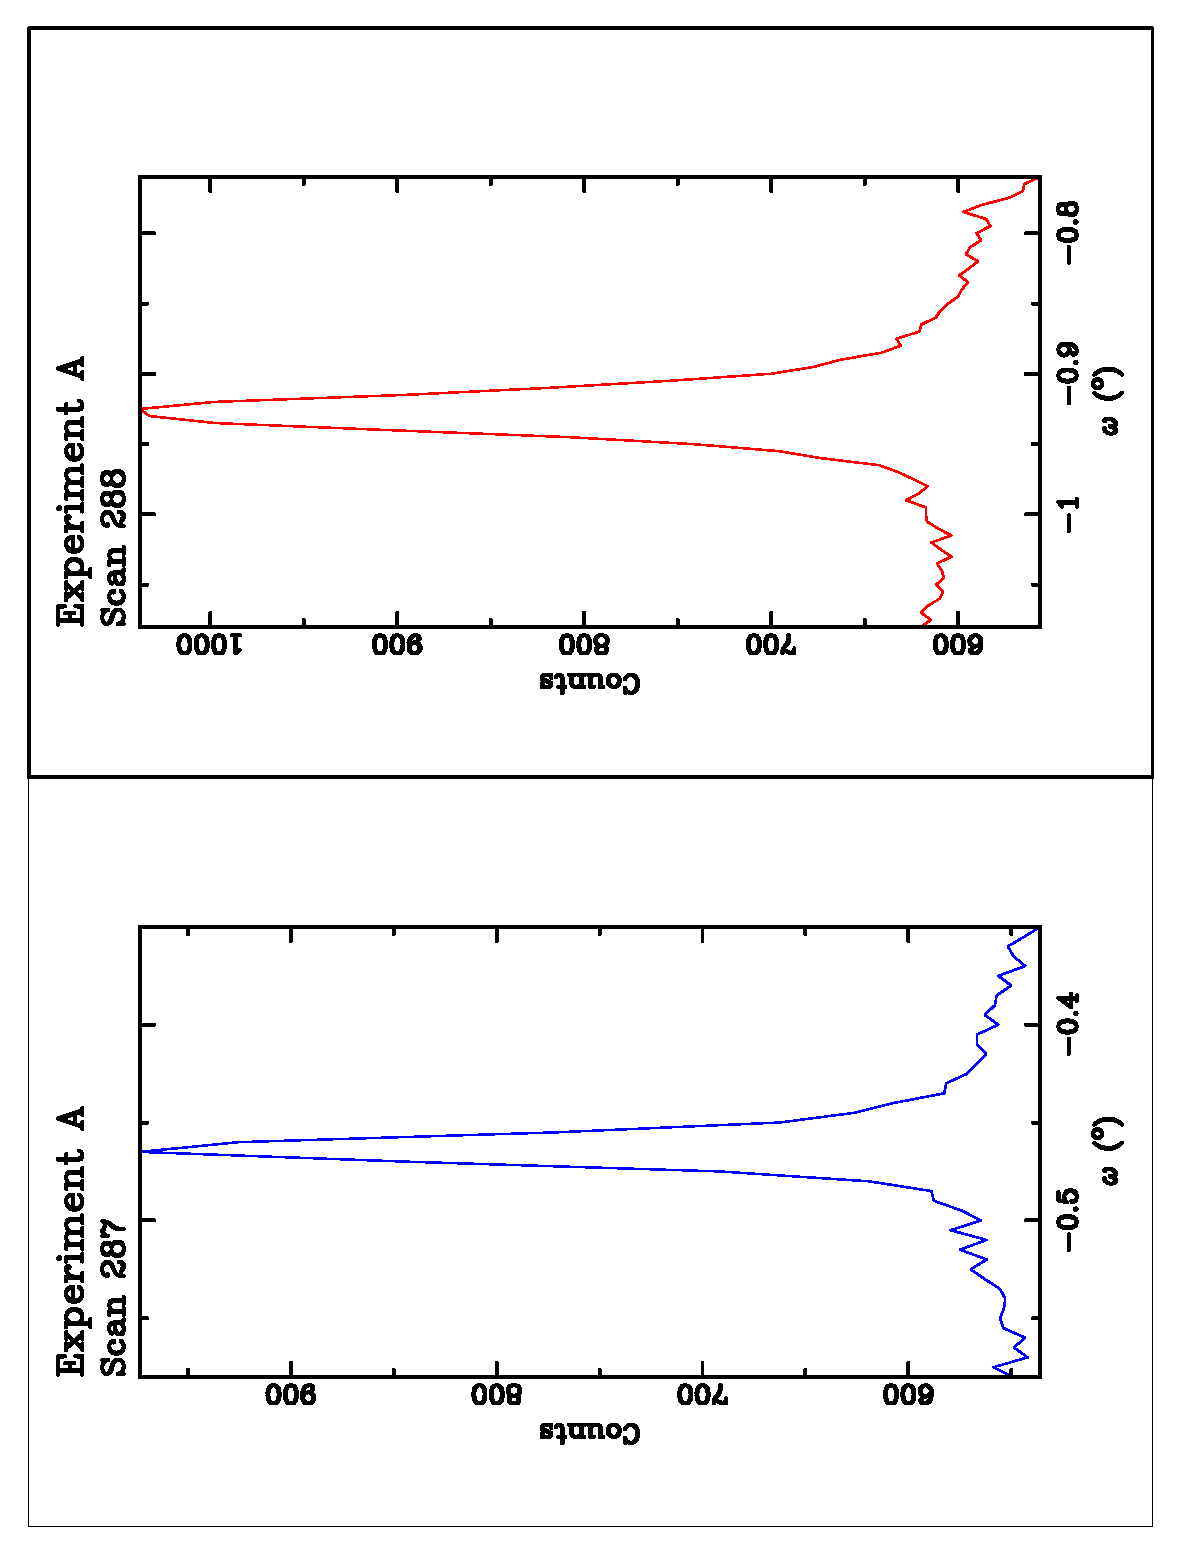
\includegraphics[scale=0.5, angle=270.0]{fra.1.eps}
   \caption{Simple example using frames}
   \label{fra-fig1}
\end{figure}

\begin{MacVerbatim}
     1  load xy,s287.xy
     2  load xy,s288.xy
     3  #
     4  tit1 Experiment A
     5  achx \gw (\uo\d)
     6  achy Counts
     7  mark 0.1,100
     8  buff 0.08
     9  fnam off
    10  fram on
    11  #
    12  nfra 2
    13  #
    14  afra 1
    15  kfra 1,1
    16  tit2 Scan 287
    17  #
    18  afra 2
    19  kfra 2,2
    20  tit2 Scan 288
    21  #
    22  plot
\end{MacVerbatim}

The macro starts with the reading of two data sets (lines 1--2).
Next title, axes labels and marker intervals are set (lines 4--7) as
in previous examples. The command 'buff' (line 8) alters the space
around the view graph reserved for axis numbering and titles. The
value is the fraction of the total width or height of the plot. In
our case we reserve 8\% of the page on all four sides of the plot as
buffer space. In line 9 the plotting of the filename is disabled and
in the following line the plotting of a border around each frame is
enabled. So far we have used no frame related commands and a plot at
this stage would show both data sets in a single view graph. In line
12 we then specify that we want to use two frames, i.e. have two
view graphs on our plot. At this stage, all settings from the
current plot (fram 1 in case we have used frames before) are copied
as defaults to all other frames. Entering command {\tt plot} now
would result in two equivalent view graphs side by side on the plot.
Thus all setting that are common to all frames should be made {\it
before} the command {\tt nfra} is used. Now we need to customize the
two frames. The command {\tt afra} determines for which frame the
following commands are used. First we alter settings for frame 1 by
entering {\tt afra 1} (line 14). Next we specify that this frame
should only contain the data from data set one (line 15) and we
enter an individual second title line (line 16). The same procedure
is repeated for frame 2 (lines 18--22) which should include data set
2 and a different subtitle line. The command {\tt plot} (line 22)
will result in a picture similar to the one in Figure
\ref{fra-fig1}.

\begin{table}[!tbh]
\centering
\begin{tabularx}{\textwidth}{|l|X|}
  \hline
  {\bf Command} & {\bf Description} \\
  \hline\hline
   afra & Sets the active frame for user input \\
   bfra & Sets background color for specified frame \\
   cfra & Copies frame parameters \\
   fram & Defines if a border is plotted around each frame \\
   kfra & Defines contents of frames (data sets or text) \\
   nfra & Sets number of frames (default = 1) \\
   sfra & Defines position and size of a frame \\
  \hline
\end{tabularx}
\caption{\label{fra-tab1}{\it KUPLOT} commands related to frames}
\end{table}

The usage of frames is rather simple and most {\it KUPLOT} settings
are individual settings for the different frames. All frame related
commands are summarized in table \ref{fra-tab1}. The following two
sections contain more complex examples using frames.

%------------------------------------------------------------------------

\section{Example 1: Using two different y-axes \label{frame-exa1}}

In this example, we will use frames to produce a plot that uses two
different y-axes to display two different data sets.  One y-axis
labeling will be on the left hand side of the view graph, the other
one on the right hand side.  The resulting plot is shown in figure
\ref{fra-fig2}. Here we display the scaling factor $f$ (right axis)
and the background parameter $b$ (left axis) of a Reverse Monte
Carlo refinement as function of the cycle number as an example plot.

\begin{figure}[!tb]
   \centering
   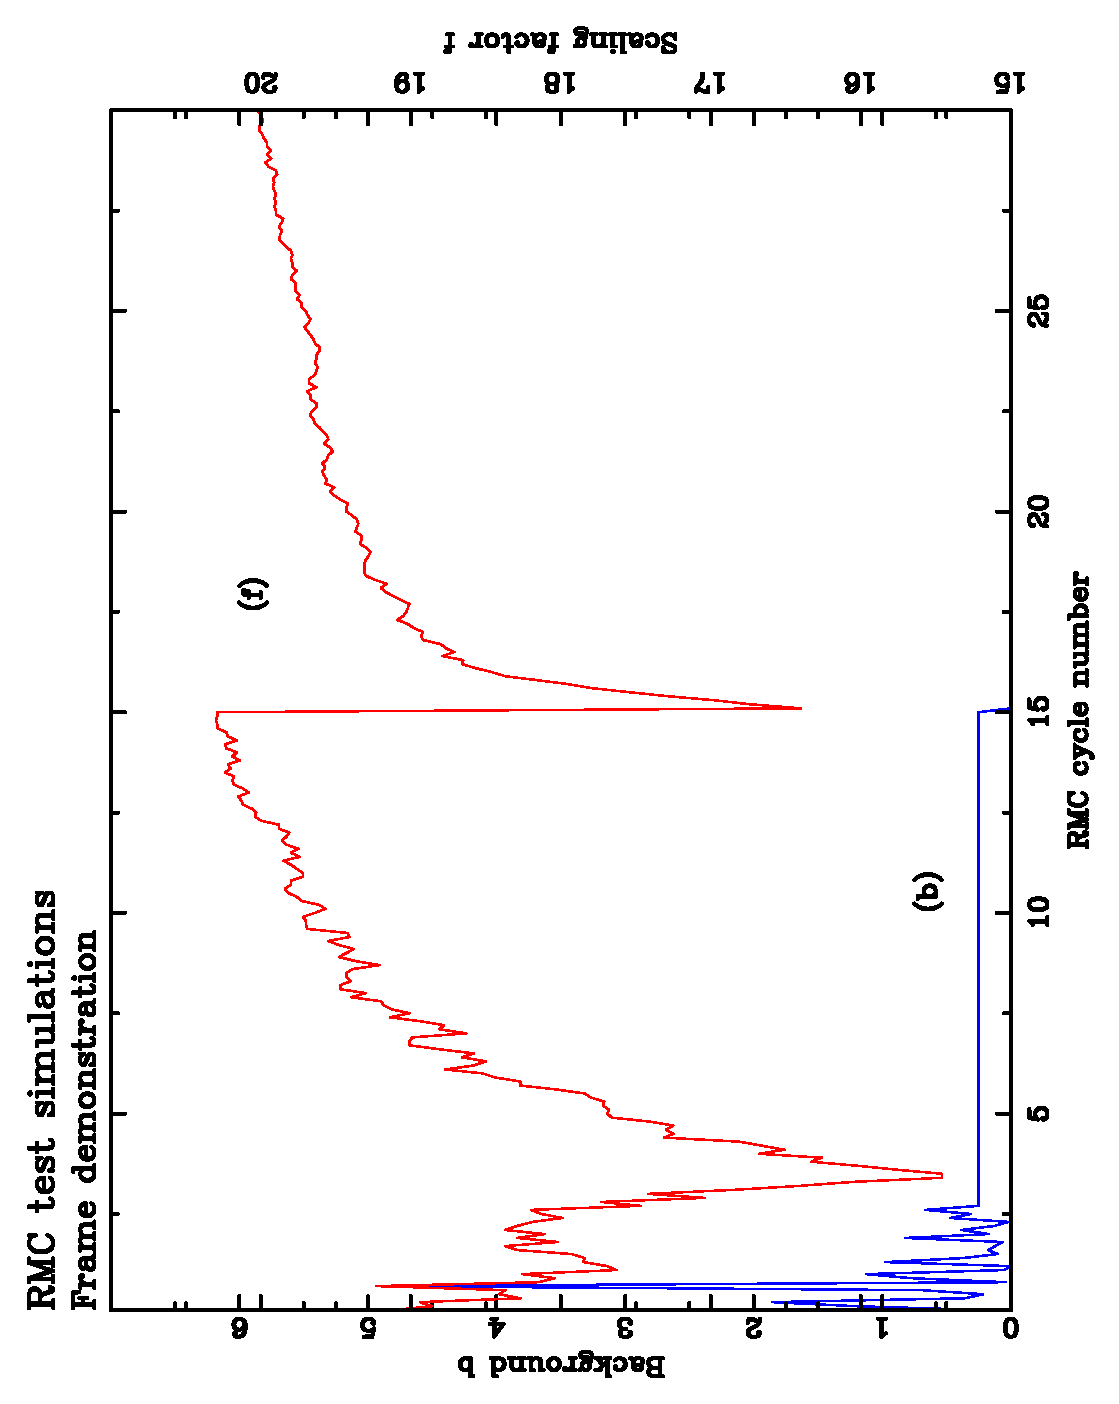
\includegraphics[scale=0.5, angle=270.0]{fra.2.eps}
   \caption{Using different y-axis with frames}
   \label{fra-fig2}
\end{figure}

We will discuss the corresponding macro file listed below step by
step. Again the line numbers are not actually part of the macro.
Lines 1--6 are nothing special, we read the two data files and set
common features like title lines.  Next we set the number of frames
to two (line 8). Since we want to plot the two data sets on top of
each other using just a different y-axes, we have to overwrite the
default location of the frames using the {\tt sfra} command (lines
10--11). The coordinates of the plot area range from 0.0 to 1.0 in
x- and y-direction. In our example both frames cover the complete
plot area.

\begin{MacVerbatim}
     1  load xy,back.xy
     2  load xy,scal.xy
     3  #
     4  fnam off
     5  tit1 RMC test simulations
     6  tit2 Frame demonstration
     7  #
     8  nfra 2
     9  #
    10  sfra 1,0.0,0.0,1.0,1.0
    11  sfra 2,0.0,0.0,1.0,1.0
    12  #
\end{MacVerbatim}

The next step is to input the settings for both frames. First we set
the input focus to frame 1 (line 13) and specify data set 1 to be
used in that frame (line 14). The {\tt fset} command in line 15
determines the layout of the view graph and setting number 3 is the
default plot layout, i.e. box, labels and tick marks in x- and
y-direction and lines at $x=0, y=0$. Finally we set the size of the
plotting window (line 16), the tick mark intervals (line 17) and the
labels for the axes (lines 18--19).

\begin{MacVerbatim}
    13  afra 1
    14  kfra 1,1
    15  fset 3
    16  skal 0.1,30.0,0.0,7.0
    17  mark 5.0,1.0
    18  achx RMC cycle number
    19  achy Background b
    20  #
\end{MacVerbatim}

The same as before has to be done for the second frame.  Lines
21--22 set the focus to the second frame and select data set 2 to be
displayed.  The negative value of the parameter of the {\tt fset}
command (line 23) indicates that the y-axis label and numbers are to
be plotted on the right hand side rather than on the left hand side
which is the default.  Again the extend of the plotting window and
the tick marks are set (lines 24--25).  Note that we need to specify
the same plotting range ($0.1 \rightarrow 30.0$) in x-direction and
a different one in y-direction compared to the settings of frame 1.
The x-axis label is switched off (line 26) because we have already
the label from the other frame.  The y-axis needs a new label (line
27).  Finally we define two annotations (line 28--29).  Note that
the given coordinates are with respect to the scaling of frame 2.

\begin{MacVerbatim}
    21  afra 2
    22  kfra 2,2
    23  fset -3
    24  skal 0.1,30.0,15.0,21.0
    25  mark 5.0,1.0
    26  achx
    27  achy Scaling factor f
    28  sann 1,"(b)",10.0,15.5
    29  sann 2,"(f)",17.5,20.0
    30  #
    31  plot
\end{MacVerbatim}

Obviously the same plot could have been achieved by scaling one of
the data sets to the y-range of the other, but the information about
the original range of y-values of one of the data sets would have
been lost in the plot in contrast to the example using frames given
here.

%------------------------------------------------------------------------

\section{Example 2: Connected view graphs \label{frame-exa2}}

In this section we will learn how we can create plots where several
graphs share one or more sides. This is done using the command {\tt
buff} we have used in the first part of this chapter. An example
plot is shown in Figure \ref{fra-fig3}.

\begin{figure}[!b]
   \centering
   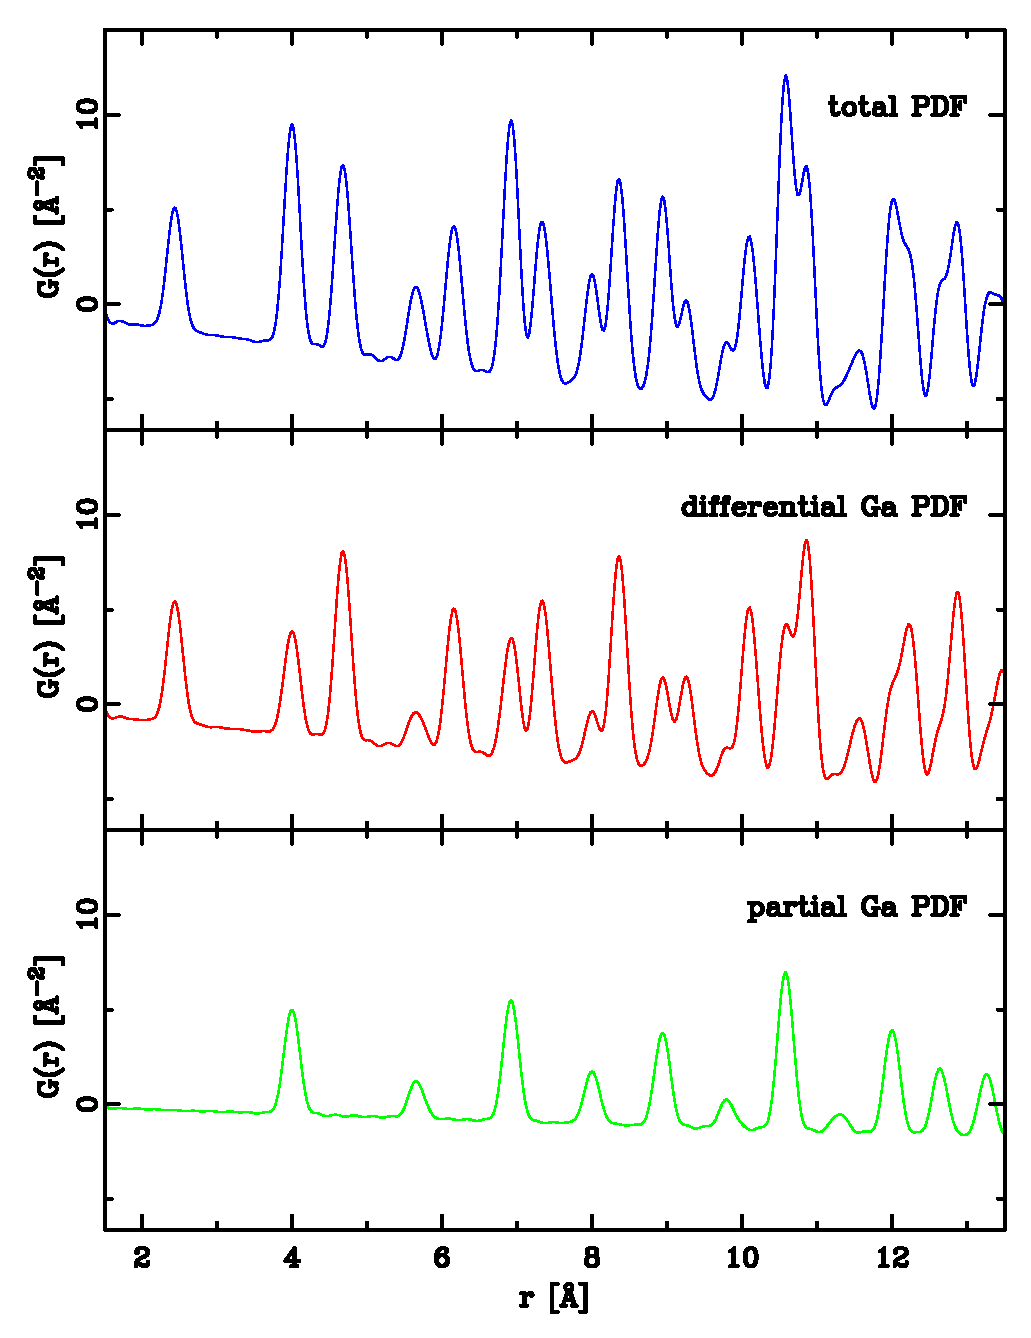
\includegraphics[scale=0.7, angle=0.0]{fra.3.eps}
   \caption{Example for connected view graphs}
   \label{fra-fig3}
\end{figure}

The macro used to create the plot is displayed below. As usual we start
resetting {\it KUPLOT} (line 1) and we select portrait orientation for
this plot (line 2). Next the data sets are loaded (lines 4--7).  This is
followed by general settings (lines 8--12) since all our frames will have
the save y-axis label, plot window and tick mark interval.

\begin{MacVerbatim}
      1  rese
      2  orient port
      3  #
      4  load xy,tot.calc
      5  load xy,dif_ga.calc
      6  load xy,par_ga.calc
      7  #
      8  fnam off
      9  fset 2
     10  achy G(r) [\A\u-2\d]
     11  skal xmin[1],xmax[1],1.2*ymin[1],1.2*ymax[1]
     12  mark 2.0,10.0
\end{MacVerbatim}

Next we define the frames, three on top of each other with no gap in
between them. Since the middle frame will have no buffer space on
the bottom and top we need to make it smaller in order for the plot
area to have the same size. Here we use variables for the task. The
value of the buffer size for title and axes labels is stored in {\tt
r[1]} (line 14), here 0.1. The remaining plot space for each panel
is calculated and stored in {\tt r[2]} (line 15). It is simply the
full size (1.0) minus two times the buffer size for the title of the
top panel and the axis label and numbering of the bottom panel. Next
we select three frames (line 17) and set the frame corners using the
variables we just defined. The $x$-range for all panels is 0.0 to
1.0. The $y$ ranges are determined by simply adding the heights of
the panels and the buffering space together (lines 18--20). Simply
calculate the numbers and it becomes clear.

\begin{MacVerbatim}
     13  #
     14  r[1] = 0.1
     15  r[2] = (1.0-2.0*r[1])/3.0
     16  #
     17  nfra 3
     18  sfra 1,0.0,2.0*r[2]+r[1],1.0,3.0*r[2]+2.0*r[1]
     19  sfra 2,0.0,    r[2]+r[1],1.0,2.0*r[2]+    r[1]
     20  sfra 3,0.0,0.0          ,1.0,    r[2]+    r[1]
\end{MacVerbatim}

In the next section the setting for the individual frames are
entered. Most of the commands were already discussed in the previous
chapters. The command {\tt buff} can either be used with a single
parameter like in the example in section \ref{frame-int} in which
case the buffer space around the view graph is the same in all
directions. Alternatively one can supply four parameters for the
required free space on the left and right side and the bottom and
top of the view graph, respectively. In our example this first frame
located on the top will have no buffer space at the bottom (line
23). Apparently we have to turn the numbering for the x-axis off
(line 25). Now we repeat the settings for the other two frames. For
the middle frame we have no buffer space on the top an bottom (line
29) and for the bottom frame we have only buffer space at the bottom
(line 34). Also we need to set a x-axis label for the bottom panel
(line 38).

\begin{MacVerbatim}
     21  #
     22  afra 1
     23  buff 0.1,0.1,0.0,r[1]
     24  kfra 1,1
     25  achx OFF
     26  sann 1,"total PDF",13.0,10.0,right
     27  #
     28  afra 2
     29  buff 0.1,0.1,0.0,0.0
     30  kfra 2,2
     31  achx OFF
     32  sann 1,"differential Ga PDF",13.0,10.0,right
     33  #
     34  afra 3
     35  buff 0.1,0.1,r[1],0.0
     36  kfra 3,3
     37  sann 1,"partial Ga PDF",13.0,10.0,right
     38  achx r [\A]
\end{MacVerbatim}

Frames are a flexible tool and can be placed anywhere on the plot
area and may also overlap. A even slightly more complex example using
frames is discussed in the next section.

%------------------------------------------------------------------------

\section{Example 3: Advanced frame usage \label{frame-exa3}}

The final example for the usage of frames is more complex and the
resulting plot is shown in Figure \ref{fra-fig4}. {\it KUPLOT} is
capable of creating quite complex plots and e.g. allows one to create
complete transparencies for a talk.

\begin{figure}[!p]
   \centering
   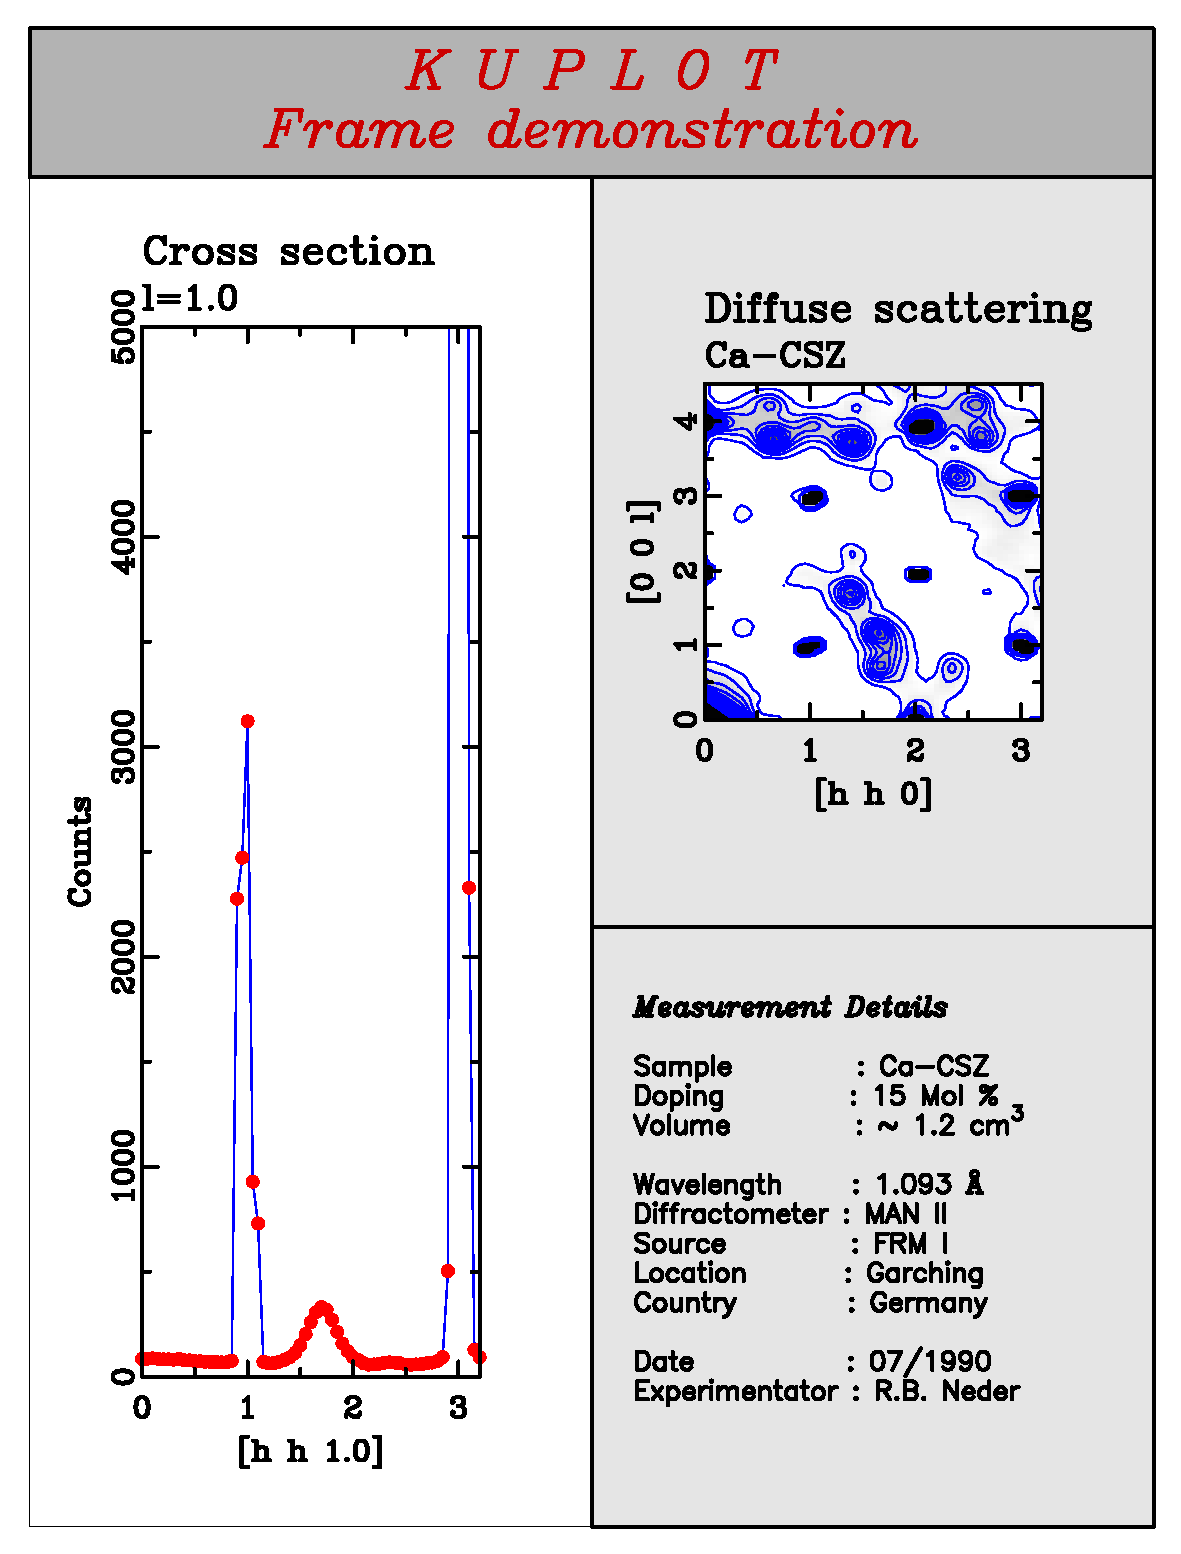
\includegraphics[scale=0.75]{fra.4.eps}
   \caption{Advanced frame example plot}
   \label{fra-fig4}
\end{figure}

The macro used to create the plot is displayed below. As usual the
data sets are loaded first (lines 1--2) followed by general
settings (line 4). Next we select 4 frames (line 6) and define the
desired frame layout (lines 8--11) and individual background
colors for each frame (lines 13--15). Note that the default
background color is white. The colors are given as RGB (red,
green, blue) values ranging from 0.0 to 1.0.

\begin{MacVerbatim}
     1  load xy,test.cut
     2  load ni,test.nipl
     3  #
     4  fnam off
     5  #
     6  nfra 4
     7  #
     8  sfra 1,0.0,0.0,0.5,0.9
     9  sfra 2,0.5,0.4,1.0,0.9
    10  sfra 3,0.5,0.0,1.0,0.4
    11  sfra 4,0.0,0.9,1.0,1.0
    12  #
    13  bfra 2,0.9,0.9,0.9
    14  bfra 3,0.9,0.9,0.9
    15  bfra 4,0.7,0.7,0.7
\end{MacVerbatim}

The next part of the macro file contains the settings for frame 1.
After setting the focus to this frame (line 19), data set 1 is
selected for this frame (line 20). The following commands specify
various settings and were already explained in previous examples.
The {\tt font} command in line 32 increases the font size of all
fonts used for this frame by 10\%.

\begin{MacVerbatim}
    16  #
    17  # Frame 1 with cross section
    18  #
    19  afra 1
    20  kfra 1,1
    21  buff 0.4
    22  lcol 1,6
    23  mtyp 1,3
    24  mcol 1,1
    25  msiz 1,0.2
    26  skal 0.0,3.2,0.0,5000.0
    27  mark 1,1000
    28  achx [h h 1.0]
    29  achy Counts
    30  tit1 Cross section
    31  tit2 l=1.0
    32  font size,1.1
\end{MacVerbatim}

Next we have the settings for frame 2 containing the 2D data set
number 2, the diffuse neutron scattering of Ca-CSZ we used as example
before. Again the various commands were  explained in earlier examples.

\begin{MacVerbatim}
    33  #
    34  # Frame 2 with data plot
    35  #
    36  afra 2
    37  kfra 2,2
    38  glat 2,3
    39  hart 2,3
    40  hcol 2,1,3
    41  hlin 1,100,50,12
    42  mark 1,1,0,0
    43  aver 0.707
    44  achx [h h 0]
    45  achy [0 0 l]
    46  tit1 Diffuse scattering
    47  tit2 Ca-CSZ
    48  font size,1.1
\end{MacVerbatim}

The next frame contains text rather than data.  The text for this
frame is read from the file {\it ref.txt} which contains exactly the
text you can see at the bottom right corner of the plot in Figure
\ref{fra-fig4}.  In lines 52--56 the justification of the text, the
font type and font size are specified. The text file may contain the
same special characters and control sequences discussed in section
\ref{1d-char}.

\begin{MacVerbatim}
    49  #
    50  # Frame 3 with text
    51  #
    52  afra 3
    53  kfra 3,ref.txt
    54  font just,left
    55  font typ,5,1
    56  font siz,5,12
\end{MacVerbatim}

Finally we specify another text file containing the title line of
the plot. We select the text to be centered (line 62) and set the
font to {\it italics} (font 3), set the color to dark red (pen 7)
and increase the size of the font to 24 points.

\begin{MacVerbatim}
    57  #
    58  # Frame 4 with title text
    59  #
    60  afra 4
    61  kfra 4,tit.txt
    62  font just,center
    63  font typ,5,3
    64  font col,5,7
    65  font siz,5,24
\end{MacVerbatim}

Currently one has not much control about the layout in a frame containing
text but that might change in future version of the program {\it KUPLOT}.

%------------------------------------------------------------------------
